% For compatibility with acroread version 
\pdfminorversion=4

\documentclass[mathserif, aspectratio=169]{beamer}
\mode<presentation>

%\usefonttheme[onlymath]{serif}
\usepackage[T1]{fontenc}
%\usepackage{tgheros}
%\usepackage{tgadventor}
%\usepackage{libertine}
%\usepackage{theinhart}
%\usepackage{palatino}
%\usepackage{newtxtext} %Times font only for text

% Use my theme
\usetheme{rognes}

% Misc packages
\usepackage{graphicx}
\usepackage[export]{adjustbox}
\usepackage{stmaryrd}
\usepackage{tikz}
\usepackage{booktabs}
\usepackage{multirow}
\usetikzlibrary{arrows,shapes,backgrounds,decorations,mindmap,patterns,snakes}
\usepackage{amsmath, amssymb, amsthm, amscd}
\usepackage[english]{babel}
\usepackage{algorithm}
\usepackage{pythonhighlight}
\usepackage{epstopdf}
\usepackage{multimedia}
\usepackage{soul}

\newcommand{\R}{\mathbb{R}}
\DeclareMathOperator{\Div}{\mathrm{div}}
\DeclareMathOperator{\Curl}{\mathrm{curl}}
\DeclareMathOperator{\Grad}{\mathrm{grad}}
\DeclareMathOperator{\D}{d}
\newcommand{\foralls}{\forall \;}
\newcommand{\iinner}[2]{\llangle #1, #2 \rrangle}
\newcommand{\inner}[2]{\langle #1,  #2\rangle}
\newcommand{\totald}{\mathrm{d}}
\newcommand{\refer}[1]{\begin{flushright}{\tiny \textcolor{darkgray}{[#1]}}\end{flushright}}
\newcommand{\referinline}[1]{{\tiny \textcolor{darkgray}{[#1]}}}
\newcommand{\ddt}[1]{{#1}_t}
\newcommand{\Mi}{M_i}
\newcommand{\Me}{M_e}
\newcommand{\Iion}{I_{\rm{ion}}}
\newcommand{\dx}{\, \mathrm{d}x}
\newcommand{\ds}{\, \mathrm{d} s}
\newcommand{\triang}{\mathcal{T}}
\DeclareMathOperator{\trace}{tr}
\newcommand{\duality}[2]{\langle #1, #2 \rangle}

\newcommand{\mysection}[1]{\begin{frame} \begin{center} \vspace{3em} \textbf{#1} \end{center} \end{frame}}
\newcommand{\sectionwithrefer}[2]{\begin{frame} \begin{center} \vspace{3em} \textbf{#1} \end{center} \refer{#2} \end{frame}}

\newtheorem{prop}[theorem]{Proposition}


\tikzstyle{na} = [baseline=-.5ex]
\tikzstyle{every picture}+=[remember picture]
\everymath{\displaystyle}

\usepackage[footnotesize, figurename=,size=scriptsize,font={color=rognesblue}]{caption}
%-------------------------------------------------------------------------------
%-------------------------------------------------------------------------------

\DeclareMathOperator{\ssum}{\textstyle \sum}

\begin{document}

%-------------------------------------------------------------------------------
\cleanpage
\begin{frame}
  \begin{columns}
    \begin{column}{0.25\textwidth}
    \centering
    \vspace{1em}
    
\includegraphics[width=\textwidth]{graphics/simula_logo_main_RGB.pdf} \\
    \vspace{1em}
    
\includegraphics[width=\textwidth]{graphics/waterscales.pdf}  \\
    \vspace{1em}
    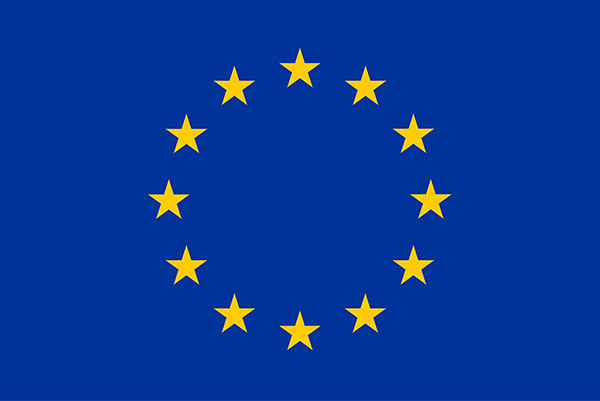
\includegraphics[height=0.3\textwidth]{graphics/flag_yellow_low.jpg} 
    \hspace{0.2em}
    
\includegraphics[width=0.3\textwidth]{graphics/logo-erc.jpg} \\
    \vspace{1em}
    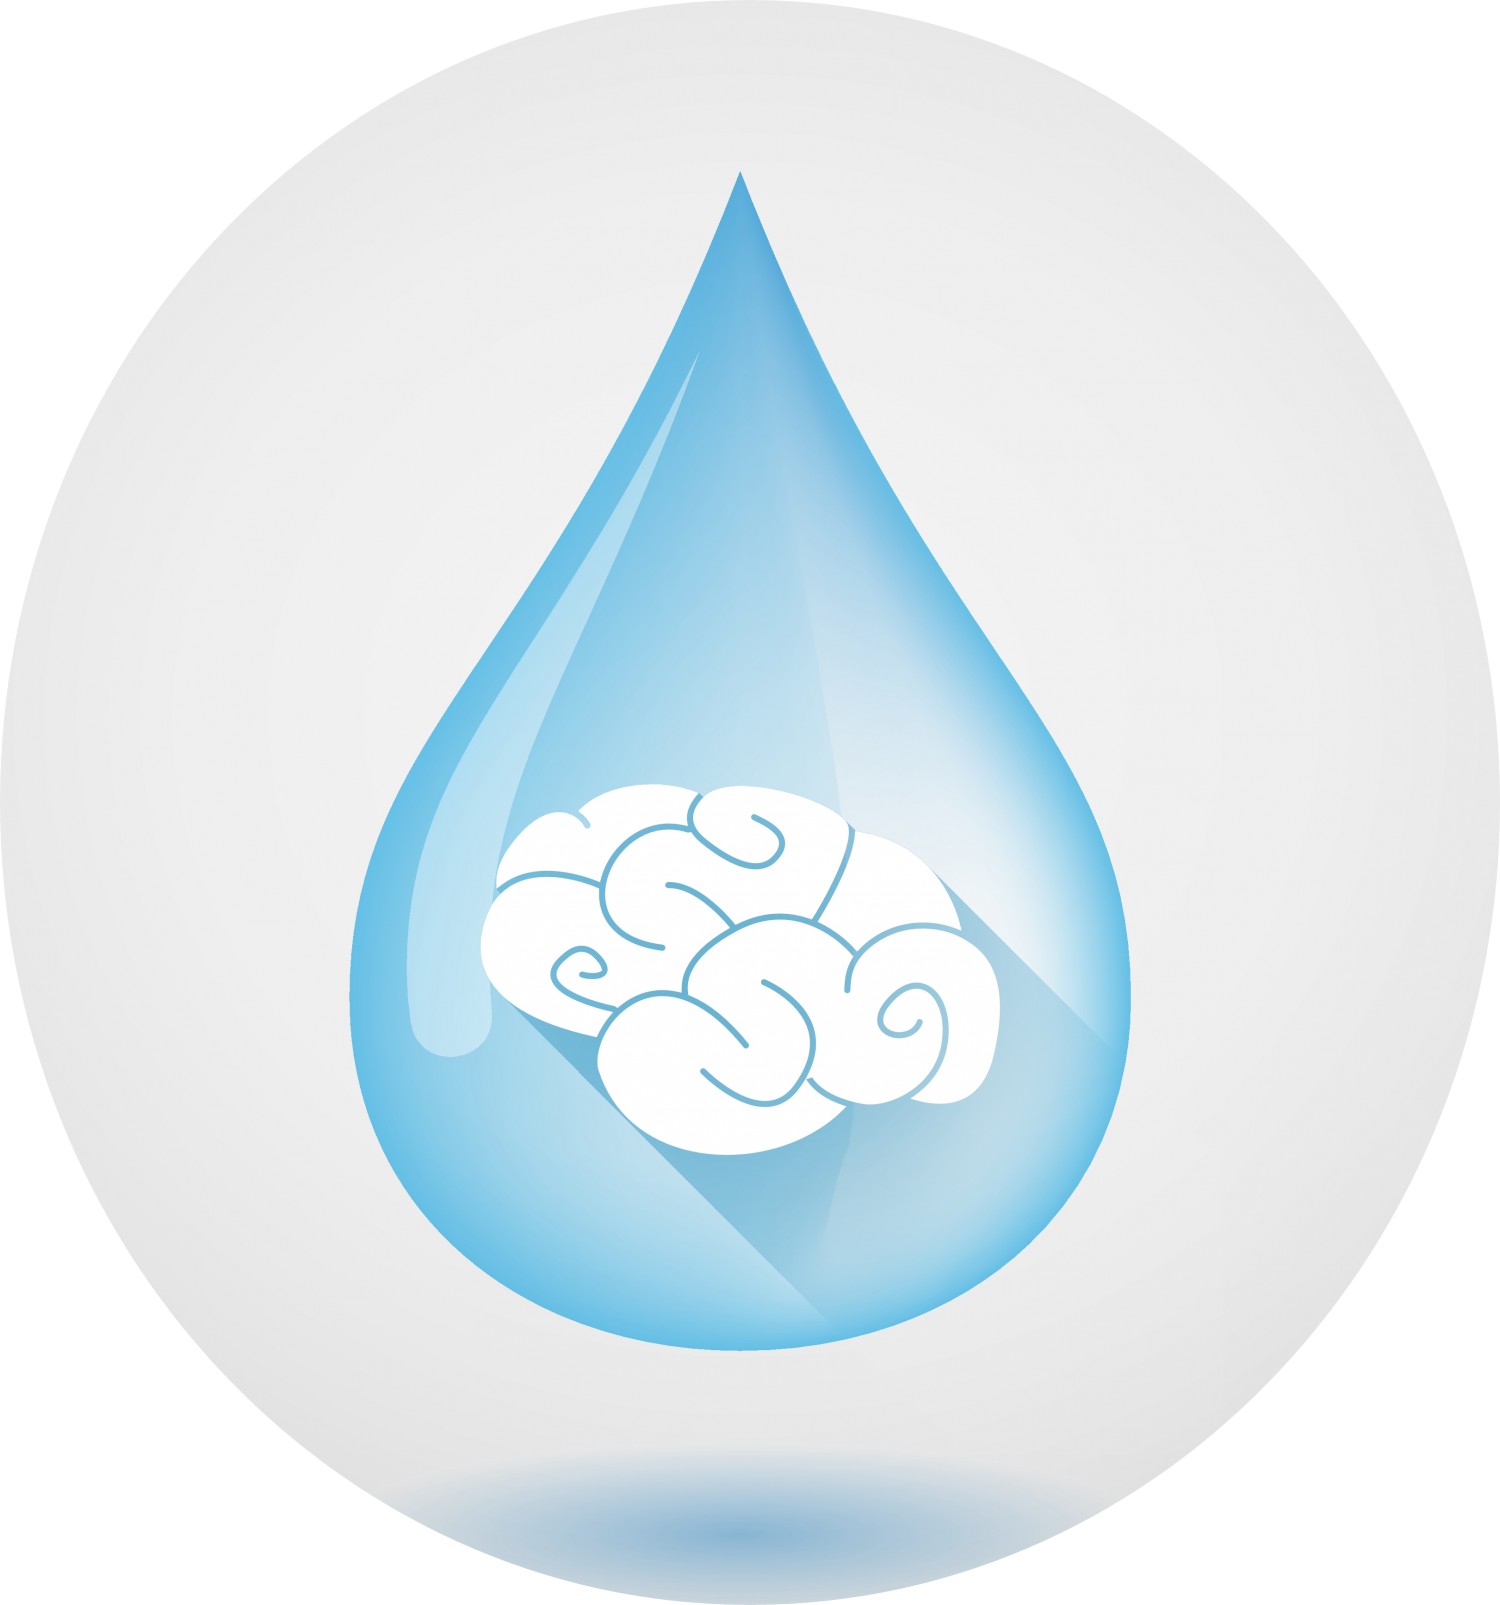
\includegraphics[width=0.5\textwidth]{graphics/waterscape_logo.png} \\
    \vspace{1em}
    
\includegraphics[width=\textwidth]{graphics/rcn-logo.pdf} \\
    \end{column}
    \begin{column}{0.75\textwidth}
    {
    \centering

      \vspace{4em}

      {\bf Mathematical modelling of the brain's waterscape} \\

      \bigskip
      \bigskip
      
      Marie E. Rognes \\
      \bigskip
      \bigskip

      Oslo, Norway \\
      \medskip
      Feb 11 2020 \\
      }
    \end{column}
  \end{columns}
\end{frame}

\cleanpage

\begin{frame}
\frametitle{Teasers from own research}

\begin{itemize}
\item
  UQ paper
\item
  MPET paper
\item
  Respiratory paper
\end{itemize}
\end{frame}


{\usebackgroundtemplate{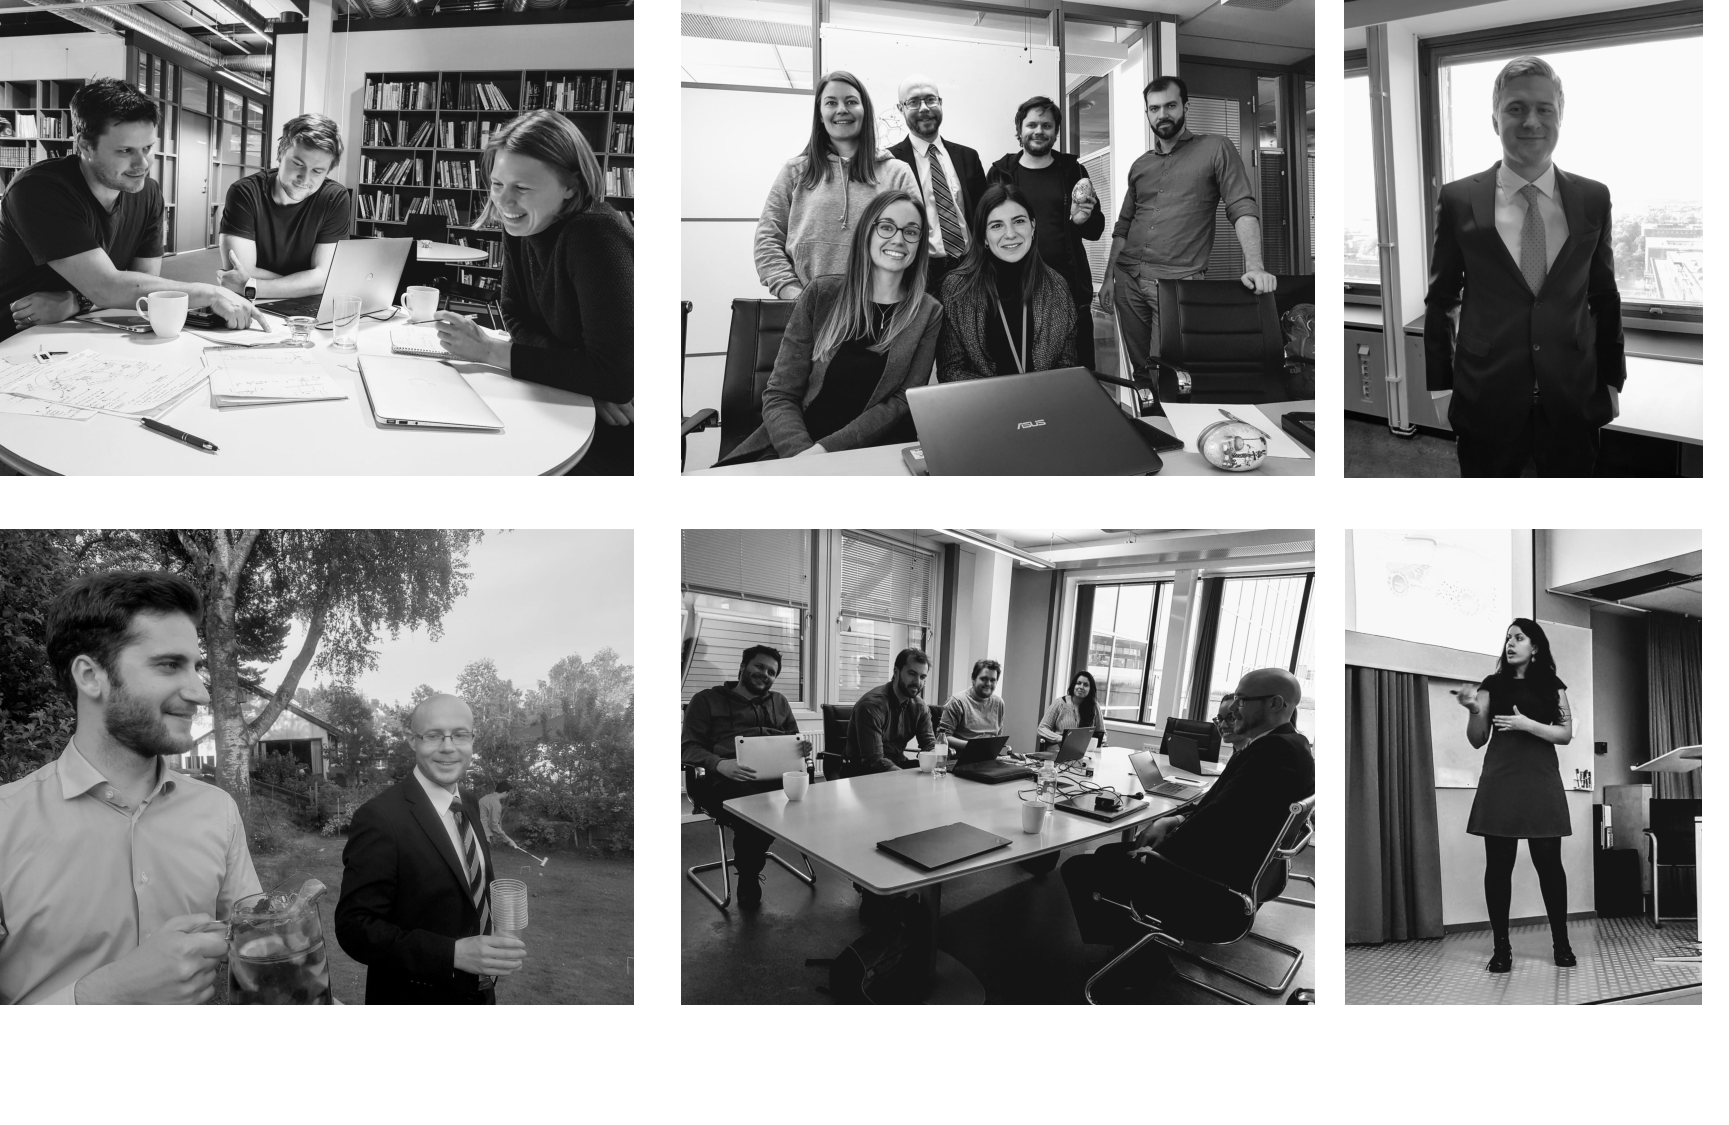
\includegraphics[width=\paperwidth]{/home/meg/presentations/slides/graphics/Collaborators.pdf}}
\begin{frame}
\end{frame}
}


\begin{frame}
  \frametitle{Outline of lectures}
  \begin{description}
    \item[Lecture 1]
      \begin{itemize}
      \item
        Why simulate the brain's waterscape?
      \item
        Where can I find the slides (and book, data, scripts)?
      \item
        Introduction to brain physiology
      \item
        Introduction to brain imaging
      \end{itemize}
    \item[Lecture 2] 
    \item[Lecture 3]
    \item[Lecture 4]
    \item[Lecture 5]
    \item[Lecture 6]
  \end{description}

%\end{enumerate}
\end{frame}

\begin{frame}
  \frametitle{Where can I find resources associated with these lectures?}
  \begin{enumerate}
  \item
    The book on GitHub
  \item
    Zenodo community:
  \end{enumerate}
\end{frame}

%
% Lecture 1
% \input{lecture1.tex}
%

\mysection{Introduction to brain anatomy}

\begin{frame}
  \frametitle{Brain anatomy: macro-scale}
\end{frame}

\begin{frame}
  \frametitle{Brain anatomy: meso-scale}
\end{frame}

\begin{frame}
  \frametitle{Brain anatomy: micro-scale}
\end{frame}

\begin{frame}
  \frametitle{Magnetic resonance imaging}
\end{frame}

\mysection{Introduction to brain physiology}

\mysection{Introduction to magnetic resonance imaging of the brain}

\begin{frame}
  \frametitle{Magnetic resonance imaging: T1 vs T2}
\end{frame}

\begin{frame}
  \frametitle{Magnetic resonance imaging: DTI}
\end{frame}

\begin{frame}
  \frametitle{Viewing and working with MRI data sets}
\end{frame}

\begin{frame}
  \frametitle{DicomBrowser and example}
\end{frame}

%-------------------------------------------------------------------------------


\end{document}
